\documentclass[border=0.2cm]{standalone}
\usepackage{tikz}

\begin{document}


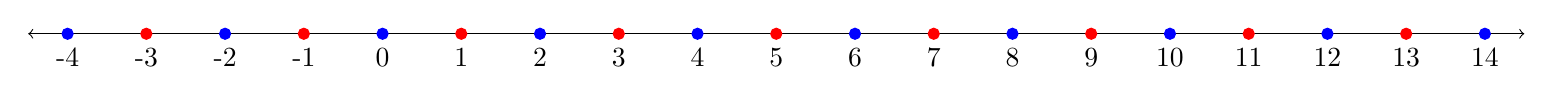
\begin{tikzpicture}
% Desenha a linha horizontal
\draw (-4,0) -- (10,0);

% Desenha setas nas duas pontas
\draw[<->] (-8.5,0) -- (10.5,0);


% Define a distância entre os elementos (1cm)
\pgfmathsetmacro{\distance}{1}

% Define o número de elementos
\pgfmathsetmacro{\numElements}{14}

% Loop para desenhar os números e setas
\foreach \i in {-4,...,\numElements} {

% Calcula a posição do elemento atual
\pgfmathsetmacro{\xPos}{-4 + \i * \distance}
  
% Desenha o número
\node at (\xPos,-0.3) {\i};
  
% Alterna entre círculo preenchido e vazio
\ifodd\i
  \filldraw[red] (\xPos,0) circle (2pt);
\else
  \filldraw[blue] (\xPos,0) circle (2pt);
\fi
}

\end{tikzpicture}
\end{document}